\section{频散与波场偏移精确度}
\label{sec:4.3}

频散系由不同频率成分以不同速度传播而形成。虽然许多读者可能听到过冰在冻结的湖
面和河面上滑动时的声音,可是在日常生活中却很少听说到频散物理现象。正在破裂的冰所
引起的弹性波,它的传播就具有频散性质,使得破裂声变成敲击震动的调子。地震波沿地表
面传播时一般可观察到波散,但对内部发生的反射波则简直很难察觉到有波散现象。在地震
数据处理中,频散是一种讨厌的事,对于处理的设计者来说,频散现象是严重的妨害和困
扰。频散现象主要由有限差分方法形成,因为微分算子和差分算子在高频上并不一致.进行
更加密的采样总可以压制掉频散,检查是否这样作了,正是生产分析人员的任务。图\ref{fig:dspr/freqdisp}
所示是某些经过频散的脉冲。

\begin{figure}[H]
\centering
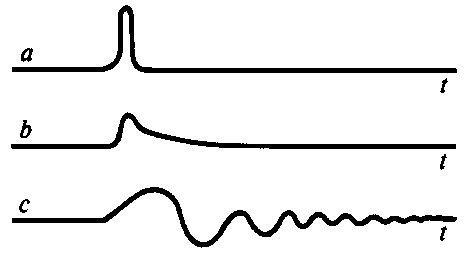
\includegraphics[width=0.65\textwidth]{dspr/freqdisp}
\caption[freqdisp]{(a)脉冲。(b)稍微频散的脉冲,因高频耗散而形成。
(c)具有显著频散的脉冲,这类频散可以因数据处理不小心而形成}
\label{fig:dspr/freqdisp}
\end{figure}

由数据处理所引起的频散可以是关于数据正处于发
生假频的危险之中的一种很有用的警告。各种频率域方
法均不依靠差分算子,所以它们都有不会表现出频散现
象的好处,不过这种好处也有附带的后果,即(1)没
有频散只限于恒定盼物质性质和(2)没有关于频散的
警告迹象就出现了空间假频。

图\ref{fig:dspr/taner}是偏移资料中出现频散的例子,上图为共
深度点叠加剖面。中间的图是处理之后的剖面,处理时
尚未企图控制频散现象,200号炮点附近在4秒时间上存
在有严重的频散现象。下面的图则是经过重新处理之后
的剖面,频散现象已大大减弱。

\begin{figure}[H]
\centering
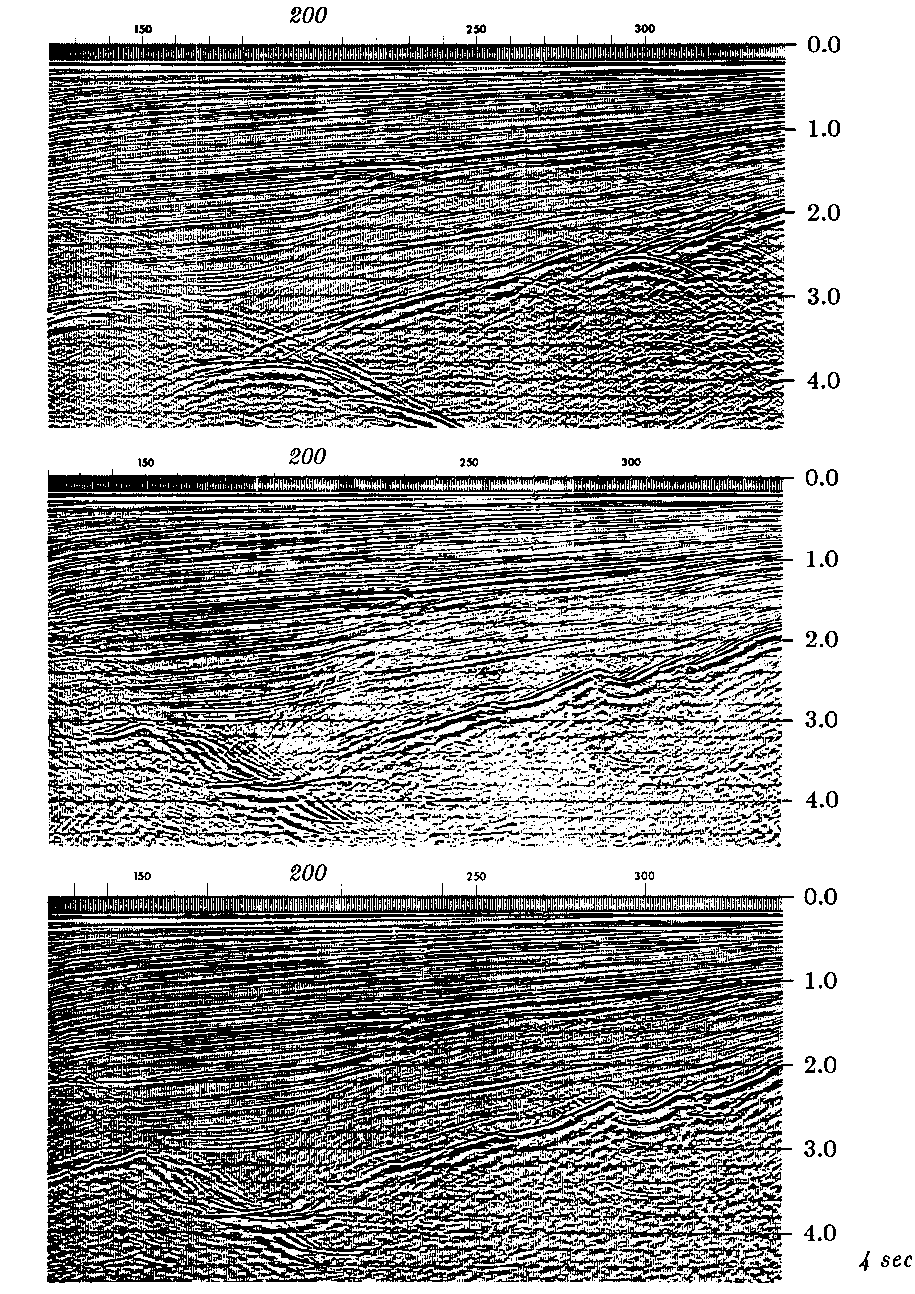
\includegraphics[width=0.65\textwidth]{dspr/taner}
\caption[taner]{克服和控制频散现象(据Taner与Koehler)}
\label{fig:dspr/taner}
\end{figure}

\subsection{空间假频}
\label{sec:4.3.1}

在时间轴上、深度轴上,检波点、炮点、中心点、炮检距或相交测线上,都会出现假
频。在水平空间坐标轴上,假频最为严重,\ref{sec:1.3}节的图\ref{fig:omk/alias}提供了一个例子,看这个图时,
关于是向左倾还是向右倾,你得到是混乱的概念,数学分析也览如此。波动方程的弥散关系
使我们能够利用半圆关系$k_z(\omega,k_x)=\sqrt{\omega^2/v^2-k_x^2}$从瞬时频率$\omega$,
速度$v$和水平空间波数
$k_x$计算出垂直空间波数$k_x$。在$x$坐标轴上进行采样时,令$k_x$的上限等于
Nyquist频率$\pi/\Delta x$。频率域方法和有限差分方法部要在处理高频时考虑到
在Nyquist频率上发生折叠的问题,
所以半圆形的频散关系在高于Nyguist频率时是折转的,如图\ref{fig:dspr/kxalias}所示。

\begin{figure}[H]
\centering
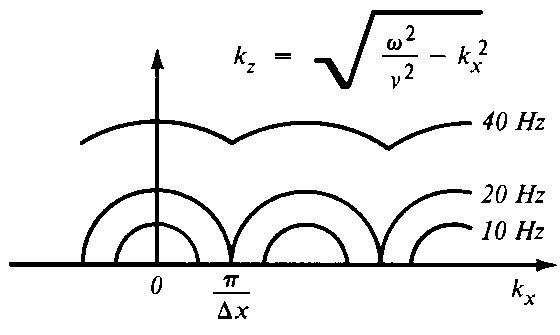
\includegraphics[width=0.65\textwidth]{dspr/kxalias}
\caption[kxalias]{对水平坐标采样时的波动方程有效频散关系,图中所示各
频率是按典型的零炮检距偏移给出的}
\label{fig:dspr/kxalias}
\end{figure}

当如图\ref{fig:dspr/kxalias}中20赫兹时的情形、
即两个圆彼此接触时,就开始有
空间假频问题了,这种情形出现在半
波长$v/2f$等于空间采样间隔$\Delta x$时。
爆炸反射面模型隐含承认所用速度应
为岩石速度的二分之一,因而,如果
条件$2f\Delta x < \frac{1}{2}v_{rock}$
能满足,假频问题就可避免了。就速度等于2公里/秒
的情形来说,保险的频率如下表所列:
\begin{table}[!ht]
\centering
\ttfamily
\small
\begin{tabularx}{\textwidth}{|Y|Y|Y|}
\hline
 & $\Delta x$ & 保险频率\\
\hline
标准情形& 25 m & <20 Hz\\
\hline
普查时& 50 m & <10 Hz\\
\hline
三维相交测线& 100 m & <5 Hz\\
\hline
\end{tabularx}
\end{table}

有关空间假频问题的另一种看法
是:陡倾斜低视速度的波可用检波器 组合方法压制(这种看法忽视炮点空
间假频)。根据这种观点,应该把能量从资料中消失时的射线角度考虑为是一个限度,超过
它空间假频就开始起作用。射线角度不取90°而取为30°时,水平波长增一倍,因此,对于
30°的射线角度和2公里/秒的速度,能保证不受假频影响的频率范围应如下表所列:
\begin{table}[!ht]
\centering
\ttfamily
\small
\begin{tabularx}{\textwidth}{|Y|Y|Y|}
\hline
 & $\Delta x$ & 保险频率\\
\hline
标准情形& 25 m & <40 Hz\\
\hline
普查时& 50 m & <20 Hz\\
\hline
三维相交测线& 100 m & <10 Hz\\
\hline
\end{tabularx}
\end{table}

因为资料通常有高于40赫兹的信号,所以广角
处理往往因有空间假频而遭致失败。

空间假频问题通常掩盖了
15°方程与90°方程之间的差别。受假频影响的能量并不在双曲线两翼与
顶点之间移动,往往停留原地不动。图\ref{fig:dspr/fdvrso}可说
明这种现象,该图表示由有限差分方程产生的90°
双曲线与15°双曲线。总的来说,它们差别很小。
注意双曲线初至的振幅,它们衰减得比球形扩散和
倾斜函数所预料的还要快,这是因为各波散曲线半
圆彼此重叠之故。这里可以不存在超出上限的传播
角度(超过该上限即产生沿x方向的假频现象)。由于波不可能达到如此之陡,所以它们确
实并不陡,脉冲也并非散布适当。

\begin{figure}[H]
\centering
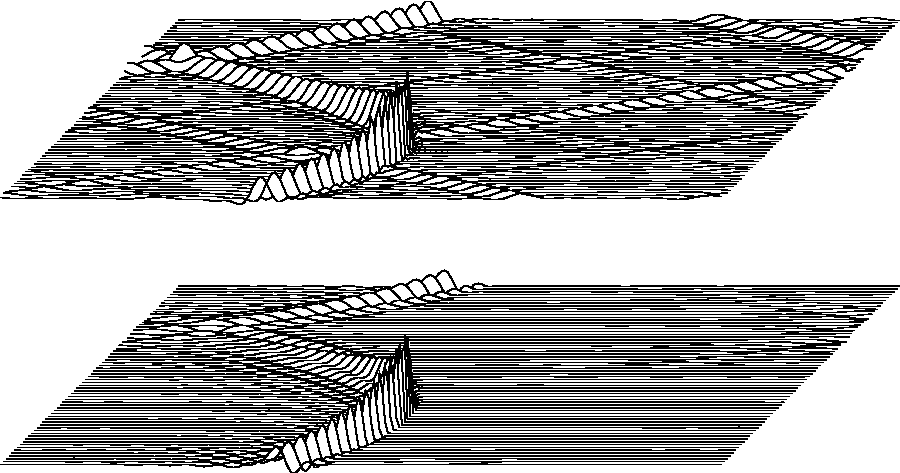
\includegraphics[width=0.65\textwidth]{dspr/fdvrso}
\caption[fdvrso]{一对合成双曲线,$\Delta t=4$毫秒,$\Delta x=25$米,
速度为2公里/秒。采用Fourier变换方法的90°方程的双曲线(上图)及15°有限差分方程的
双曲线(下图)}
\label{fig:dspr/fdvrso}
\end{figure}

\subsection{二阶空间导数 }
\label{sec:4.3.2}

二阶差分算子的定义方程为
\begin{equation}
\frac{\delta^2}{\delta x^2}P=\frac{P(x+\Delta x)-2P(x)+P(x-\Delta x)}{(\Delta x)^2}
\label{eq:ex4.3.1}
\end{equation}
取下列极限则可定义二阶导数算子
\begin{equation}
\frac{\partial^2}{\partial x^2}P=\lim_{\Delta \to 0}\frac{\delta^2}{\delta x^2}P
\label{eq:ex4.3.2}
\end{equation}
$\Delta x$趋于零时,许多不同的定义可以全部趋于相同的极限。问题在于要求出一种表达式,该表
达式当$\Delta x$大于零时应是准确的,而且,按某种实用水平衡量,该表达式还不得过于复杂。我
们第一个目标就是要知道方程\ref{eq:ex4.3.1}的精确度如何能定量计算,第二个目标就是要考虑一
种比方程\ref{eq:ex4.3.1}稍微复杂一点但比它更精确得多的表达式。

我们将采用的基本分析方法是Fourier变换。取复指数的导数$P=P_0\exp(ikx)$,并将
任何误差均考虑为空间波数的函数,对于二阶导数,有
\begin{equation}
\frac{\partial^2}{\partial x^2}P=-k^2P
\label{eq:ex4.3.3}
\end{equation}
用类似于差分算子的表达式来定义$\hat{k}$
\begin{equation}
\frac{\delta^2}{\delta x^2}P=-\hat{k^2}P
\label{eq:ex4.3.4}
\end{equation}
理想情形是$\hat{k}$要等于k。将复指数$P_0\exp(ikx)=P$代入式\ref{eq:ex4.3.1},
可看到由定义式\ref{eq:ex4.3.4}得出以$k$表示的一种有关$k$之表达式
\begin{subequations}
\begin{equation}
-\hat{k^2}P=\frac{P_0}{(\Delta x)^2}[e^{ik(x+\Delta x)}-2e^{ikx}+e^{ik(x-\Delta x)}]
\label{eq:ex4.3.5a}
\end{equation}
\begin{equation}
-\frac{\delta^2}{\delta x^2}=\hat{k^2}=\frac{2}{(\Delta x)^2}[1-\cos(k\Delta x)]
\label{eq:ex4.3.5b}
\end{equation}
\label{eq:ex4.3.5}
根据式\ref{eq:ex4.3.5b}作出$\hat{k}\Delta x$对$k\Delta x$的关系图,是很直接了当的事。三角学的半角公式允
许我们取式\ref{eq:ex4.3.5b}的解析平方根,得
\begin{equation}
\frac{\hat{k}\Delta x}{2}=\sin\frac{k\Delta x}{2}
\label{eq:ex4.3.5c}
\end{equation}
\end{subequations}
作级数展开之后将表明,在低频情形下,$\hat{k}$确实是能很好地近似于$k$,在Nyquist频率上,
根据定义$k\Delta x=\pi$,所得近似$\hat{k}\Delta x=2$则是对于$\pi$的一种很坏的近似。


\subsection{1/6策略}
\label{sec:4.3.3}

减小$\Delta x$,恒可提高绝对精度。增加较高阶项,例如
\begin{equation}
\frac{\partial^2}{\partial x^2}\approx\frac{\delta^2}{\delta x^2}
-\frac{\Delta x^2}{12}\frac{\delta^4}{\delta x^4}+\text{等等}
\label{eq:ex4.3.6}
\end{equation}
则需要以增加计算机时间和分析时的麻烦为代价,换得提高与Nyquist频率有关的精度。当
$\Delta x$趋于零时,方程\ref{eq:ex4.3.6}趋于基本定义式\ref{eq:ex4.3.1}和\ref{eq:ex4.3.2}。
如果希望在$k$值小时有
高精度,可以用Taylor级数方法决定式\ref{eq:ex4.3.6}中像1/12这类的系数。或者,如果希望在
办值的某种范围内有一定精度,可以用曲线拟合方法来确定稍微有点不同的系数。在实际处
理中,极少采用式\ref{eq:ex4.3.6},因为还有一种不太明显的表达式能以很少代价就可提供高得
多的精度!这种思想可用下式简要说明:
\begin{subequations}
\begin{equation}
\frac{\partial^2}{\partial x^2}\approx
\frac{\frac{\delta^2}{\delta x^2}}{1+b\Delta x^2\frac{\delta^2}{\delta x^2}}
\label{eq:ex4.3.7a}
\end{equation}
式中,$b$是一个可调常数。
将式\ref{eq:ex4.3.5b}代入,得
\begin{equation}
(\frac{\hat{k}\Delta x}{2})^2=
\frac{\sin^2(\frac{k\Delta x}{2})}{1-b4\sin^2(\frac{k\Delta x}{2})}
\label{eq:ex4.3.7b}
\end{equation}
\label{eq:ex4.3.7}
\end{subequations}
就能对式\ref{eq:ex4.3.7a}的精度作出数值估计。在取值$b=
1/6$的情形下,对上式取平方根的计算结果绘于图\ref{fig:dspr/sixth}。

\begin{figure}[H]
\centering
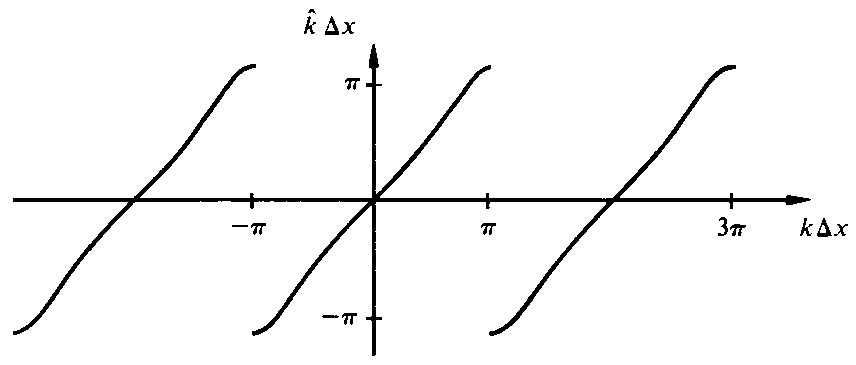
\includegraphics[width=0.65\textwidth]{dspr/sixth}
\caption[sixth]{作为空间波数之函数的二阶导数表示式\ref{eq:ex4.3.7}的精度
式\ref{eq:ex4.3.7b}之平方根的符号在$-\pi$至$\pi$满范围内取成与$k$一致,而在该范围
之外则为周期性质(据Hale)}
\label{fig:dspr/sixth}
\end{figure}

若式\ref{eq:ex4.3.7}内的系数1/6
以1/12代替。则略去高于二阶$\Delta x$的各项后,式\ref{eq:ex4.3.4}与
\ref{eq:ex4.3.7}将是一致的。系数
1/12来自级数展开,但是系数取为1/6则可适用于较宽的范围,
因而是共同采用的值。 Francis Muir曾经指出,值$1/4-1/\pi^2\approx1/6.726$
在Nyquist频率给出
严格的拟合,并且在所有低频范
围上都是准确地拟合!很少有勘
探人员考虑到,尽管式\ref{eq:ex4.3.7}还有精度不足之嫌,但已足以保证野外记录值的内插了。
图\ref{fig:dspr/sixth5}是各种不同b值之双曲线的比较,在图中可观察到,不论b值是多少,最长的波长都
是以相同的速度传播的。图\ref{fig:dspr/sixth5}中的时间轴仅有256个点的长度,而在实际工作中,它将方
有成千个以上的点。所以,图\ref{fig:dspr/sixth5}是夸大了实际工作中应归因于沿x轴进行有限差分而产生
的频散影响。

让我们确信:如何把式\ref{eq:ex4.3.7}付诸应用算是搞清楚了吧。取$b
= 6$。最简单的典型会
程是热流方程:
\begin{equation}
\frac{\partial}{\partial t}q=
\frac{\partial^2}{\partial x^2}q\approx
\frac{\frac{\delta^2}{\delta x^2}}{1+\frac{\Delta x^2}{6}
\frac{\delta^2}{\delta x^2}}q
\label{eq:ex4.3.8}
\end{equation}
由此可知,将该方程通乘以式中的分母项,得
\begin{equation}
(1+\frac{\delta x^2}{6}\frac{\delta^2}{\delta x^2})
\frac{\partial}{\partial t}q=
\frac{\partial^2}{\partial x^2}q\approx
\delta_{xx}q
\label{eq:ex4.3.9}
\end{equation}
据此即可进行计算了。

\begin{figure}[H]
\centering
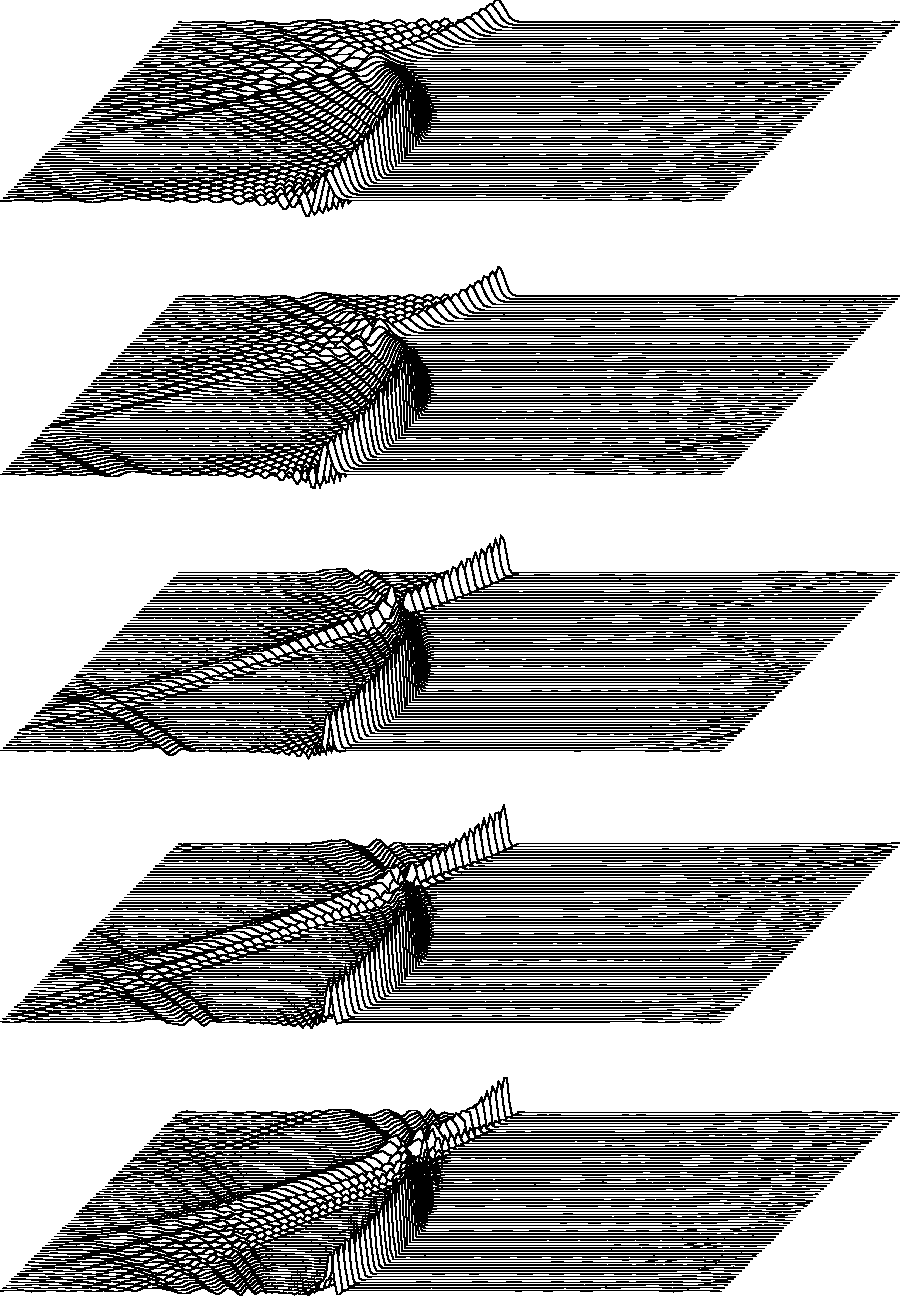
\includegraphics[width=0.65\textwidth]{dspr/sixth5}
\caption[sixth5]{ b = 0, 1/12, 1/6.726, 1/6 和l/5 情形下的双曲线}
\label{fig:dspr/sixth5}
\end{figure}

\subsection{时间导数与深度导数及双线变换}
\label{sec:4.3.4}

你很可能会认为二阶导数就是二阶导数,没什么数学理由要把时间导数作不同于空间导
数的处理。事情可不是这么回事。考虑一下边界条件,你就能受到启示,明白时间导数与空
间导数之间是有悬殊不同的,处理时间导数时(而且总是要同沿深度z的导数一起处理),
我们必须考虑因果性条件---这意味着,未来是唯一地决定于现在和过去,加在时间坐标上
的适当边界条件就是初始条件,它是该函数本身(或许还有它的某些导数)在一个点上,即
在时间初始点上的具体值,对于深度坐标z来说,那种特殊点就是时的地表面,但是横
向空间导数则有所不同:它们需要有在两个分离很远的点上的边界条件,通常这些点是在所
论体积的左侧和右侧。

微分方程
\begin{equation}
\frac{dq}{dz}=ik_z(\omega
,k_x)q
\label{eq:ex4.3.10}
\end{equation}
是与$k_z$的定义本身有联系的,类似的差分方程则将定义一个$\hat{k_z}$ :
\begin{equation}
\frac{q_{z+\Delta z}-q_z}{\Delta z}=i\hat{k_z}
\frac{q_{z+\Delta z}+q_z}{2}
\label{eq:ex4.3.11}
\end{equation}
将式\ref{eq:ex4.3.10}的解$g=g_0exp(ik_zz)$
代入式\ref{eq:ex4.3.11},使我们得到所期望的$k_z$与实际有
的$k_z$二者之间的关系:
\begin{equation}
i\hat{k_z}\Delta z=
2\frac{e^{ik_z\Delta z-1}}{e^{ik_z\Delta z+1}}=
2\frac{e^{ik_z\Delta z/2}-e^{-ik_z\Delta z/2}}
{e^{ik_z\Delta z/2}+e^{-ik_z\Delta z/2}}
\label{eq:ex4.3.12}
\end{equation}
这个关系以双线变换而著称(见\ref{sec:4. 6}节)
\begin{equation}
i\hat{k_z}\Delta z=2i\frac{\sin k_z\Delta z/2}{\cos k_z\Delta z/2}
\label{eq:ex4.3.13}
\end{equation}
\begin{equation}
\frac{\hat{k_z}\Delta z}{2}=\tan\frac{k_z\Delta z}{2}
\label{eq:ex4.3.14}
\end{equation}

式\ref{eq:ex4.3.14}给出了采用Crank-Nicolson方法所得一阶导数的精度,
回顾一下\ref{sec:2.7}节
中所述的偏移差分格式,我们曾经以完成深度差分的相同方式来完成时间差分,所以必须应
用相同的精度限制,即
\begin{equation}
\frac{\hat{\omega}\Delta t}{2}=\tan\frac{\omega \Delta t}{2}
\label{eq:ex4.3.15}
\end{equation}
作级数展开将表明,当$\Delta t$趋于零时,$\hat{\omega}$趋近于$\omega$。每个波长有4、10和20个点时的相对误差
分别为30\%, 3\%和1\%。不论是要求选取很小的$\Delta t$还是需要比式\ref{eq:ex4.3.14}更精确的方法, 这些误差都相当地大了。

可惜,看来似乎还不存在比Crank-Nicolson表示式要精确一些的满足因果性条件之微
分表示式,这里没什么像1/6策略那样的东西,这样一来就必然要根据Nyquist准则把采样间
隔$\Delta z$与$\Delta t$大大地加以减小了.也许实际景象不会像我正在描绘的那样前途暗淡吧,许多人
都对以4毫秒采样间隔$\Delta t = 4ms$进行时间域偏移的效率和精度还是满意的。

Stolt的经典论文(1978
)除了介绍快速Fourier变换偏移方法之外,还指出:降低因果
性条件的要求时可以达到更高的精度。
Stolt说明了如何在已知深度水平上使因果性条件要
求降低,而同时保持它在下一个深度水平上能进行稳定的有限差分。尽管Fourier方法能够
应用于分立的各地层,可是沿着深度的$z$坐标轴我们还是不得不同因果性微分打交道。然
而,深度坐标轴没有像测线方向x坐标轴和时间f坐标轴那样的麻烦事,因为它只影响计算时
间,并不影响数据内存。

有限差分的解并不只是要求频率近似---它们真正要达到的是对的近似。解
出式\ref{eq:ex4.3.11}的未知数,得
\begin{equation}
q_{z+\Delta z}=(\frac{1+i\hat{k_z}\Delta z/2}{1-i\hat{k_z}\Delta z/2})q_z
\label{eq:ex4.3.16}
\end{equation}
所以,在深度$z=N\Delta z$之内有$N_z$层的情形下,我们得下列近似
\begin{equation}
e^{ik_zN\Delta z}\approx(\frac{1+i\hat{k_z}\Delta z/2}{1-i\hat{k_z}\Delta z/2})^N
\label{eq:ex4.3.17}
\end{equation}
以后我们将把它用于有限差分之Fourier域模拟的程序。将在\ref{sec:4.7}节内讨论的这类模拟使我
们能够对各种不同偏移方法的精度进行比较。



